% -*-coding: utf-8 -*-

\chapter{Struktura kódu}\label{struktura kódu}

    Pro lepší pochopení souvislostí mezi třídami popisovanými v kapitole~\ref{cpu impl} uvádíme na následující straně UML diagram kompletní hierarchie tříd vytvořený aplikací Visual Paradigm for UML 8.2. Diagram obsahuje kromě dříve popisovaných tříd (modré) i další neimplementované třídy (šedé), které dohromady tvoří kostru jednoduché aplikace pro testování filtrů optimalizované ve fázi návrhu pro rychlé spouštění těchto filtrů bez zbytečné režie. Aplikace by umožnila načítání konfiguračních dat ze souboru, případné zobrazení výsledku pomocí jednoduchého grafického API. Toto budiž odpověď na otázku, jaká byla motivace zvolit právě tuto strukturu.

    V současném stavu jsou třídy {\tt Filter}, {\tt SEManager} a {\tt ImageManager} používány rovnou přímo ve funkci {\tt main} a pro nové nastavení fitrů je třeba kód znovu zkompilovat.

    Celý kód je k dispozci na přiloženém DVD.

    \section{Práce s 3D daty}

        \subsection{Uspořádání v operační paměti}

        Kvůli rychlejší alokaci, kopírování a přesunu na (z) GPU jsou 3D data v paměti serializována do jednorozměrného pole podobně jako 3D maska do vektoru vah. Rozsah (0-255) je v paměti reprezentován klasicky jako {\tt unsigned char}, rozsah (0-65535) je však reprezentován 32-bitovým typem {\tt unsigned int}, jako pokusná optimalizace na přesnost a rychlost\note{ nedat to opravdu jako 16-bit?}. Okraje obrazu (viz sekce~\ref{lokální zprac}) jsou dodefinovány nulou, šířka okrajů je neměnná a musí být známa v době alokace. Vzorová data obsahují scan mozku, který má tmavé okraje, takže nulové okraje jsou přirozené, navíc při filtraci nedochází k jejich zneplatnění a nemusí být obnovovány.

        \subsection{Formát souborů}

        3D data jsou načítána ze souboru ve formátu \Analyze, jehož specifikaci lze nalézt např. na webu \cite{Analyze 7.5}. Jedná se o dnes už zastaralý dvousouborový formát, vhodný pouze pro demonstrační účely\notea{ok?}. Soubor fname.hdr obsahuje hlavičku (rozměry, použitý datový typ, orientace...) a soubor fname.img obsahuje samotná obrazová data uspořádaná podle pokynů v hlavičce. Výstupním formátem klasické nekomprimované bmp v odstínech šedi, kde jsou 3D data uložena po řezech v předem definovaném směru, aby byla možná jednoduchá vizuální kontrola výsledků.

        \subsection{Životní cyklus dat}

        \paragraph{Načtení} dat ze souboru má na starosti metoda {\tt Load3D(fname,frameSize=-1)}, která nejprve přečte hlavičku a podle ní inicializuje (statické) členy \Imageinfo. Poté připraví příslušně velké pole datového typu \imDataType  včetně okrajů širokých {\tt frameSize} a do něj (s ohledem na okraje) uloží obrazová data přepočtená na žádaný datový typ. Je možné načíst libovolné množství vstupních souborů, inicializace geometrie však proběhne pouze podle prvního z nich, pro ostatní už se jen ověří, zda jsou rozměrově stejné a pokud ne, načítání selže. Jelikož velikost okrajů je neměnná, je nutné při načtení prvního 3D obrázku zadat {\tt frameSize} podle poleměru největší používané masky. Tato hodnota se také uloží do \Imageinfo  a není ji třeba pro další načítání zadávat. Pole s jednotlivými obrázky jsou postupně ukládána do vektoru \image  a pokud je nastavena proměnná {\tt CudaInfo::useCuda}, jsou taktéž odeslána na GPU pod příslušné složky vektoru \imageGpu.

        \paragraph{Filtrace}Pokud při ní chceme data uložit do nového obrázku, musíme použít funkci {\tt PrepareBlankImage(where,idx=-1)}, která podle parametru {\tt where} alokuje na konci příslušného vektoru (\image, nebo \imageGpu) pole příslušné velikosti a do druhého vektoru uloží pouze {\tt NULL} -- kvůli šetření pamětí (hlavně na GPU), a aby měly oba vektory stejně složek, jinak by se obrázky na CPU a GPU mohly zkřížit. Pokud chceme pouze přesunout obrázek z (na) GPU a na druhém zařízení ještě není alokované místo např. v důsledku dříve popsané oprerace, zavoláme tutéž funkci s požadovaným {\tt where} a {\tt idx} podle toho, pro jaký obrázek chceme paměť doalokovat.

        \paragraph{Ukládání} do bmp obstarává metoda {\tt SaveBmp(idx,fname,slicingDir,slicesPerLine)}. Ta udělá z 3D dat uložených v {\tt image[idx]} kolmé řezy podle hodnoty {\tt slicingDir} (0,1,2), které posléze uspořádá vedle sebe a pod sebe do 2D obrázku tak, že na řádku je právě {\tt slicesPerLine} řezů. Natočení řezů bylo nastaveno tak, aby řezy mozku (vzorová data) vypadaly rozumně. Data jsou poté přepočtena (nikoliv normalizována) do rozsahu 0-255 a uložena jako jednokanálové bmp s paletou v odstínech šedi. Pokud jsou data k uložení na GPU, je třeba je napřed zkopírovat do RAM.


    \section{Maska}
        \subsection{Načítání a práce s maskou}

        Nejprve se v konstruktoru {\tt SEManager} vytvoří překladový \bq slovník\eq~-- pole o stejné velikosti a formátu jako {\tt maska[]} obsahující rozdíly indexů do pole obrazu. K tomu je třeba znát geometrii obrázku a {\tt SEManager} tak může být konkretizován až po načtení prvního z nich.

        O načtení masky ze zmíněného formátu se pak stará funkce {\tt Parse2SE(name,mask)}, kde {\tt name} je ukazatel na typ {\tt string} a {\tt mask} ukazatel na pole ve stejném formátu jako {\tt maska[]}. Funkce přidá do vektoru {\tt sE} další prvek {\tt structEl*}, vyplní jméno, vstupní pole {\tt mask} zkopíruje do stejnojmeného atributu (pro případná další přeparsování) a {\tt wList} vyplní pole slovníku tak, že rozdíl indexů k \textit{i}-tému voxelu okolí se v něm objeví právě tolikrát, kolik je váha tohoto voxelu ve vstupním poli {\tt mask}. Délka {\tt wList} je tedy rovna kapacitě masky -- narozdíl od délky {\tt structEl::mask}, která je konstatně rovna velikosti masky.

        Poznamenejme ještě, že šířku okrajů, která se promítne do hodnot ve {\tt wList}, stanovujeme podle největší použité masky. Pokud chceme použít i menší masky, musíme je v zadání \emph{doplnit nulami do formátu největší použité masky}, abychom dostali správné výsledky. Na výkon to však vliv mít nebude, neboť {\tt wList} nezahrne prvky s nulovou vahou.

    \section{Filtry}
        \subsection{Formát funkce}

        Funkce filtrů mají jednotný formát {\tt jmého(dst,seIndex,srcA,p4)}, parametry jsou po řadě ukazatel, kam má být uložen výsledek, index použité masky a ukazatel na zdroj. Čtvrtý parametr je šablonová unie všech dalších možných parametrů -- u arimetických \bq filtrů\eq, jako sčítání a odčítání je to ukazatel na druhý obrázek, u (samostatně neimplentovaného) \kk-tého prvků by to bylo \kk ~atd. Filtry pracují cele buď na CPU, nebo GPU, tzn. všechny ukazatele na data musejí být buď z vektoru \image, nebo \imageGpu. Uvnitř všech funkcí je pak výhybka podle hodnoty {\tt CudaInfo::useCuda}, a buď je spuštěn filtr na CPU, nebo na GPU. Zda-li hodnotě {\tt CudaInfo::useCuda} odpovídají i zdrojové a cílové destinace již funkce neověřuje.

    \section{Walshův seznam na GPU}

        Walshův seznam na GPU napočítávámě efektivně tak, že nejprve paralelně pro celý blok vytvoříme ve sdílené paměti pole s dvojicemi indexů do váženého seznamu. Tyto dvojice říkají, z jakých prvků máme Walhův seznam napočítat. Samotný výpočet prvků pak provádí opět paralelně skupina vláken podle takto připraveného pole, když je to aktuálně třeba. Pole indexů je na začátku \emph{napočítáváno}, protože je to rychlejší, než ho načítat z globální paměti (kam bychom ho mohli jedině uložit).
\vfill
\newpage
\hspace{-1cm}
\begin{overpic}[width = \textheight, angle = 90]
    {src/8Appendix/diagram.pdf}
    \put(6,4){
\includegraphics{src/8Appendix/whitestrip.png}}
    \put(45,0){Obrázek A.1: UML diagram tříd v kódu}
\end{overpic}

\chapter{Grafická příloha -- příklady}\label{příloha obrázky}

    Kompletní výsledky všech filtrů pro všechny dále uvedené šumy jsou k dispozici na přiložením DVD. Pro demonstraci filtrů byla opět pouužita stejná data jako pro měření urychlení: 3D SPECT scan mozku o rozměrech $79 \times 95 \times 69$ voxelů v odstínech šedi (0-255). Pro větší zřetelnost byl z výsledku vybrán vždy jeden reprezentativní horizontální řez (konkrétně 31.).

    \section{Morfologické filtry}

    Následují ukázky filtrů dilatace, eroze a detekce hran při použití masky s poloměrem 1 a kapacitou 26 (poslední z masek na obrázku 5.1, bez centrálního voxelu). Můžeme vidět, že u detekce hran dochází kvůli nulovým okrajům na stranách obrázku k degeneraci, protože obrázek zasahuje až ke krajům -- zde by bylo vhodnější použít např. okraje s konstantním opakováním.
    \vfill
    \newpage
    \begin{figure}[htp]
        \begin{minipage}[l]{0.5\textwidth}
            \center
            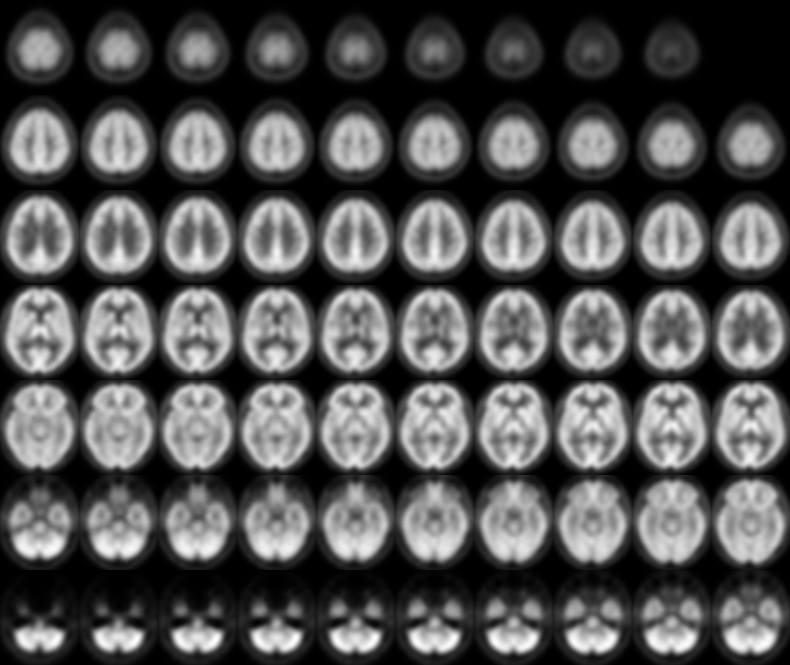
\includegraphics[width = 150pt]{src/8Appendix/final/original.png}
            \caption{Originál}
        \end{minipage}
        \begin{minipage}[r]{0.5\textwidth}
            \center
            
\includegraphics[width = 150pt]{src/8Appendix/final/dilatace.png}
            \caption{Dilatace}
        \end{minipage}
     \end{figure}
     \begin{figure}[h]
        \begin{minipage}[l]{0.5\textwidth}
            \center
            
\includegraphics[width = 150pt]{src/8Appendix/final/eroze.png}
            \caption{Eroze}
        \end{minipage}
        \begin{minipage}[r]{0.5\textwidth}
            \center
            
\includegraphics[width = 150pt]{src/8Appendix/final/hrany.png}
            \caption{Detekce hran}
        \end{minipage}
    \end{figure}


    \section{Statisticky motivované filtry}

    Rozdíly mezi filtry medián, BES, H.-L. medián a WBES předvedeme na kontaminovaném gaussovském šumu s velkou 10\% kontaminací a $\sigma = 10$ při použití datového typu {\tt usigned char}. Poté předvedeme subjektivně nejlepší výsledky (pouze jeden vítězný filtr) pro šum s kontaminací 5 \% a $\sigma = 15$ (agresivní šum) a šum s kontaminací 3 \% a $\sigma = 5$. Parametry šumů jsou poněkud nadsazené kvůli ilustraci schopností filtrů. U řezů vždy ukážeme výsledek filtrace a rozdíl oproti nepoškozenému originálu, pro lepší viditelnost inverzní a vynásobený pěti. Jako subjektivně vítězný fitr jsme pokaždé vybrali ten, kde rozdíl již neměl výrazný chrakter šumu, ale zároveň ještě nedošlo k přílišnému vyhazení (rozdíl byl stále hodně světlý).

    Byla použita maska s poloměrem 1 a kapacitou 27 (poslední na obrázku 5.1) a pro dosažení lepších výsledků maska s poloměrem 2 a kapacitou 80 (krychle $5\times 5\times 5$ bez hran a středu). Čas výpočtu WBES na CPU se pro větší masku pohyboval okolo 40s, H.-L. mediánu okolo 27s, zrychlení na GPU není známo, protože po uplynutí cca 7s bez odezvy CPU kartu resetuje. Navíc zde by byl algoritmus použitý pro tyto filtry extrémě neefektivní kvůli velikosti Walshova seznamu.

    Pro zašumění originálu byla napsána funkce {\tt AddNoise(...)}. V ní je nejprve rozhoduto zda dotyčný voxel bude kontaminovaný -- pokud ne, je pomocí Box-Mulleorvy\footnote{Umožňuje generovat dvě nezávislá N(0,1) rozdělení z dvou nezávislých U(0,1) rozdělení -- ta se dají získat pomocí fukce {\tt rand()}.} formule nagenerován šum s rozdělením N(0,1), který je posléze přetransformován a přičten k hodnotě voxelu.

    U filtrů je opět v dolním indexu uváděna kapacita masky. Samotný šum bez kontaminace uvádíme jen kvůli porovnání, filtry samozřejmě pracují s kontaminovaným šumem. Nyní výsledky pro jednotlivé šumy v pořadí, jak byly popsány (10\%/10, 5\%/15 a 3\%/5):

    \vfill
    \begin{figure}[htp]
        \center
        \begin{minipage}[c]{0.5\textwidth}
            \center
            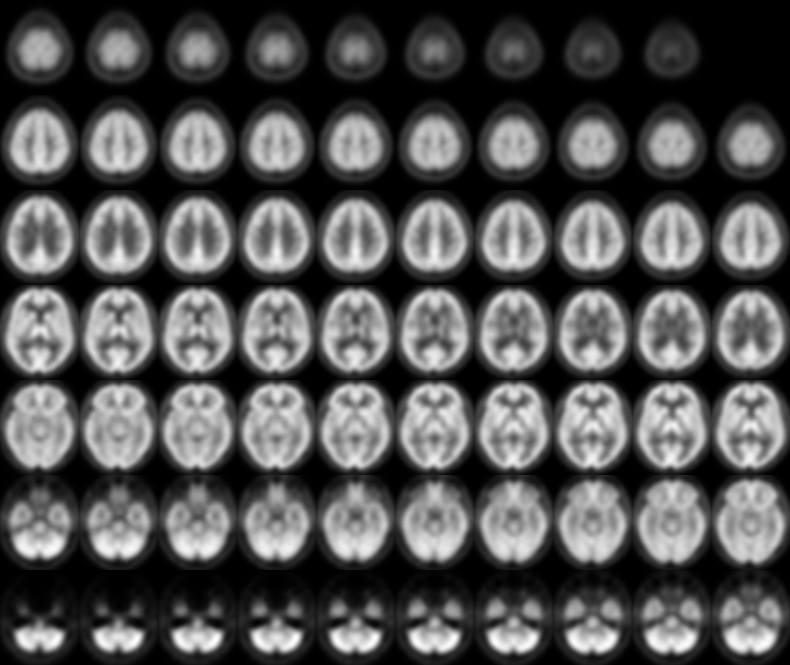
\includegraphics[width = 150pt]{src/8Appendix/final/original.png}
            \caption{Originál}
        \end{minipage}
     \end{figure}
     \begin{figure}[h]
        \begin{minipage}[l]{0.5\textwidth}
            \center
            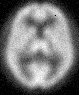
\includegraphics[width = 150pt]{src/8Appendix/final/10-100noise.png}
        \end{minipage}
        \begin{minipage}[r]{0.5\textwidth}
            \center
            
\includegraphics[width = 150pt]{src/8Appendix/final/10-100contaminated.png}
        \end{minipage}
        \\
        \begin{minipage}[l]{0.5\textwidth}
            \caption{Šum, $\sigma = 10$}
        \end{minipage}
        \begin{minipage}[r]{0.5\textwidth}
            \caption{Šum, $\sigma = 10$, kontaminace 10~\%}
        \end{minipage}
    \end{figure}

    \begin{figure}[htp]
        \begin{minipage}[l]{0.5\textwidth}
            \center
            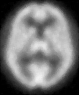
\includegraphics[width = 150pt]{src/8Appendix/final/10-100med.png}
            \caption{Medián$_{27}$}
        \end{minipage}
        \begin{minipage}[r]{0.5\textwidth}
            \center
            
\includegraphics[width = 150pt]{src/8Appendix/final/10-100medD.png}
            \caption{Medián$_{27}$ -- originál}
        \end{minipage}
        \begin{minipage}[l]{0.5\textwidth}
            \center
            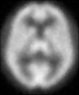
\includegraphics[width = 150pt]{src/8Appendix/final/10-100bes.png}
            \caption{BES$_{27}$}
        \end{minipage}
        \begin{minipage}[r]{0.5\textwidth}
            \center
            
\includegraphics[width = 150pt]{src/8Appendix/final/10-100besD.png}
            \caption{BES$_{27}$ -- originál}
        \end{minipage}
        \begin{minipage}[l]{0.5\textwidth}
            \center
            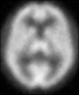
\includegraphics[width = 150pt]{src/8Appendix/final/10-100wmed.png}
            \caption{H.-L. medián$_{27}$}
        \end{minipage}
        \begin{minipage}[r]{0.5\textwidth}
            \center
            
\includegraphics[width = 150pt]{src/8Appendix/final/10-100wmedD.png}
            \caption{H.-L. Medián$_{27}$ -- originál}
        \end{minipage}
    \end{figure}
    \vfill
    \newpage
    ~\vfill~
    \begin{figure}[htp]
        \begin{minipage}[l]{0.5\textwidth}
            \center
            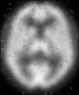
\includegraphics[width = 150pt]{src/8Appendix/final/10-100wbes.png}
            \caption{WBES$_{27}$}
        \end{minipage}
        \begin{minipage}[r]{0.5\textwidth}
            \center
            
\includegraphics[width = 150pt]{src/8Appendix/final/10-100wbesD.png}
            \caption{WBES$_{27}$ -- originál}
        \end{minipage}
    \end{figure}

    \begin{figure}[h]
        \begin{minipage}[l]{0.5\textwidth}
            \center
            
\includegraphics[width = 150pt]{src/8Appendix/final/10-100besL.png}
            \caption{BES$_{80}$ (poloměr 2, vítěz)}
        \end{minipage}
        \begin{minipage}[r]{0.5\textwidth}
            \center
            
\includegraphics[width = 150pt]{src/8Appendix/final/10-100besLD.png}
            \caption{BES$_{80}$ -- originál}
        \end{minipage}
    \end{figure}
    ~\vfill~
    \newpage

    \begin{figure}[H]
        \center
        \begin{minipage}[c]{0.5\textwidth}
            \center
            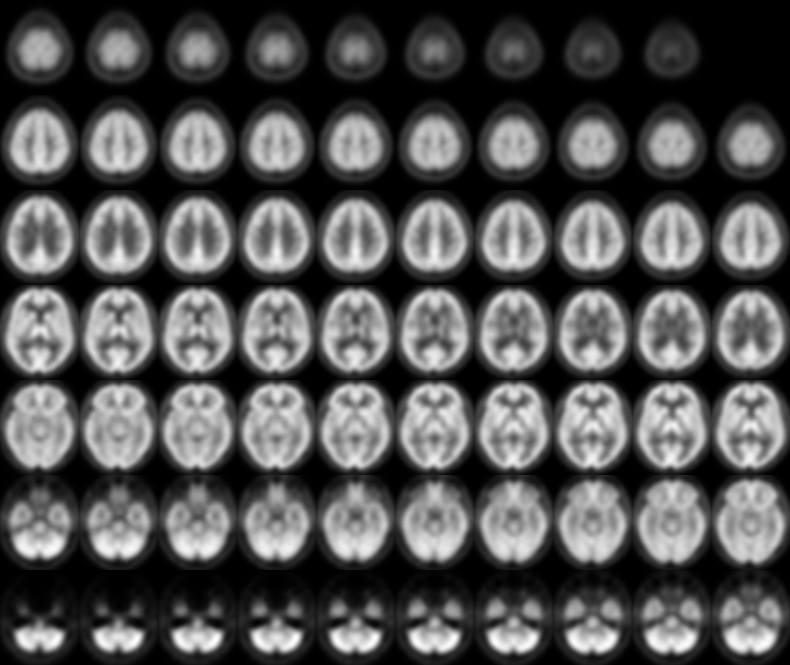
\includegraphics[width = 140pt]{src/8Appendix/final/original.png}
            \caption{Originál}
        \end{minipage}
     \end{figure}
     \begin{figure}[H]
        \begin{minipage}[l]{0.5\textwidth}
            \center
            
\includegraphics[width = 140pt]{src/8Appendix/final/15-50noise.png}
            %\caption{Zašuměný originál}
        \end{minipage}
        \begin{minipage}[r]{0.5\textwidth}
            \center
            
\includegraphics[width = 140pt]{src/8Appendix/final/15-50contaminated.png}
            %\caption{Zašuměný a kontaminovaný originál}
        \end{minipage}
        \\
        \begin{minipage}[l]{0.5\textwidth}
            \caption{Šum, $\sigma = 15$}
        \end{minipage}
        \begin{minipage}[r]{0.5\textwidth}
            \caption{Šum, $\sigma = 15$, kontaminace 5~\%}
        \end{minipage}
        \begin{minipage}[l]{0.5\textwidth}
            \center
            
\includegraphics[width = 140pt]{src/8Appendix/final/15-50wbesL.png}
            \caption{WBES$_{80}$ (poloměr 2, vítěz)}
        \end{minipage}
        \begin{minipage}[r]{0.5\textwidth}
            \center
            
\includegraphics[width = 140pt]{src/8Appendix/final/15-50wbesLD.png}
            \caption{WBES$_{80}$ -- originál}
        \end{minipage}
    \end{figure}
    \newpage
    \begin{figure}[H]
        \center
        \begin{minipage}[c]{0.5\textwidth}
            \center
            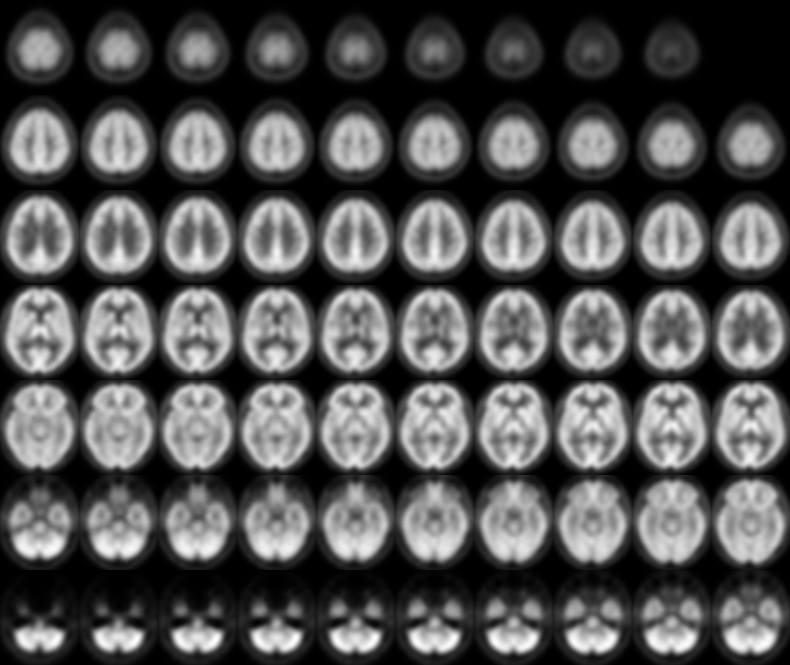
\includegraphics[width = 140pt]{src/8Appendix/final/original.png}
            \caption{Originál}
        \end{minipage}
    \end{figure}
    \begin{figure}[H]
        \begin{minipage}[l]{0.5\textwidth}
            \center
            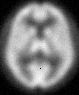
\includegraphics[width = 140pt]{src/8Appendix/final/5-30noise.png}
            %\caption{Zašuměný originál}
        \end{minipage}
        \begin{minipage}[r]{0.5\textwidth}
            \center
            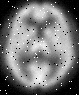
\includegraphics[width = 140pt]{src/8Appendix/final/5-30contaminated.png}
            %\caption{Zašuměný a kontaminovaný originál}
        \end{minipage}
        \\
        \begin{minipage}[l]{0.5\textwidth}
            \caption{Šum, $\sigma = 5$}
        \end{minipage}
        \begin{minipage}[r]{0.5\textwidth}
            \caption{Šum, $\sigma = 5$, kontaminace 3~\%}
        \end{minipage}
        \begin{minipage}[l]{0.5\textwidth}
            \center
            
\includegraphics[width = 140pt]{src/8Appendix/final/5-30bes.png}
            \caption{BES$_{27}$ (vítěz)}
        \end{minipage}
        \begin{minipage}[r]{0.5\textwidth}
            \center
            
\includegraphics[width = 140pt]{src/8Appendix/final/5-30besD.png}
            \caption{BES$_{27}$ -- originál}
        \end{minipage}
    \end{figure}
